%% ------------------------------------------------------------------------- %%
\chapter{Resultados}
\label{cap:resultados}

Os resultados obtidos através do processamento descrito no capítulo anterior
serão enumerados a seguir.


%% ------------------------------------------------------------------------- %%
\section{Resultados Anteriores}
\index{resultados anteriores}
\label{sec:old_results}

Antes dos resultados obtidos pelos modelos discutidos, 
serão apresentados alguns já conhecidos que poderão servir como referência ou ponto de partida.

%% ------------------------------------------------------------------------- %%
\subsection{GSHAP}
\index{GSHAP}
\label{sec:gshap}

Um dos resultados mais conhecidos de avaliação de ameaça sísmica global é o GSHAP \citep{giardini_1999}.

A figura \ref{fig:gshap} apresenta os resultados do GSHAP para América do Sul.
E escala está limitada para que sejam claras as variações no território brasileiro.

\begin{figure}[H]
  \centering
  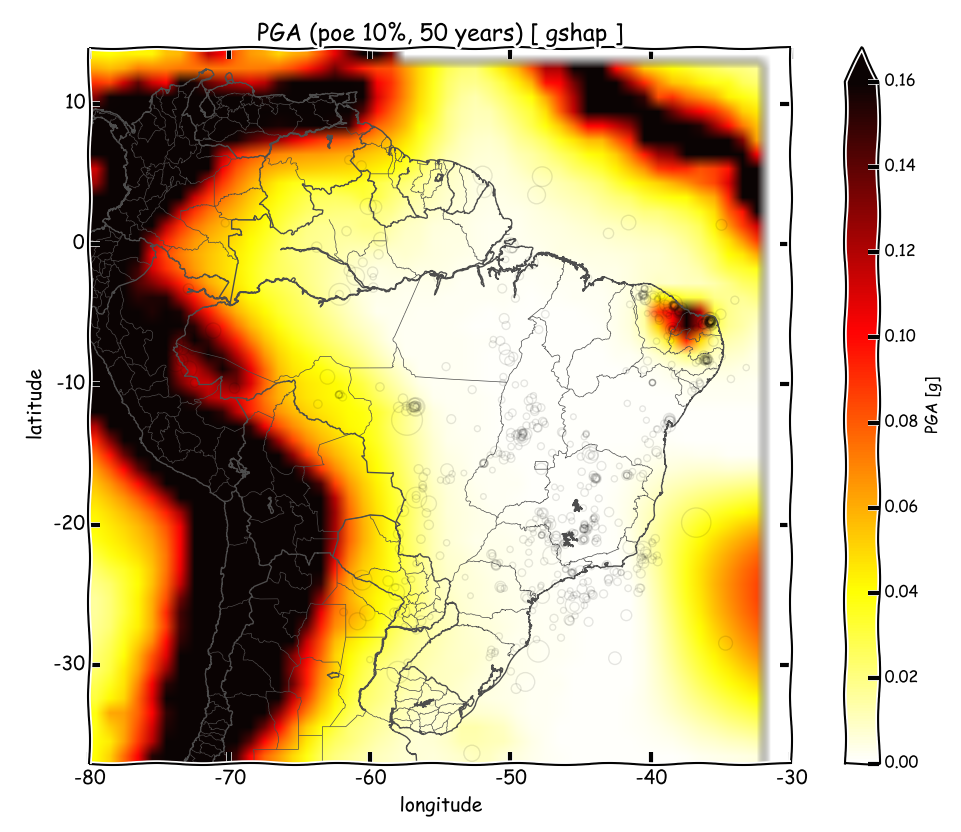
\includegraphics[width=.80\textwidth]{pga_gshap} 
  \caption{Resultado do GSHAP para o Brasil: \gls{PGA} (10\%/50anos) em unidades de $g$}
  \label{fig:gshap} 
\end{figure}

É possível observar no GSHAP a grande influência de sismos provenientes da zona de subdução nos Andes 
sob o território do Acre. Também é destacada a sismicidade no Nordeste, com um pico de 0.16g para a PGA, e por
último, chama a atenção o resto do país por haver um vazio de informação.


%% ------------------------------------------------------------------------- %%
\subsection{Zoneamento Sísmico}
\index{zoneamento}
\label{sec:zonning}

Existem também esforços \citep{dourado_2014} para se criar um modelo para a ameaça sísmica brasileira
usando a metodologia clássica de Cornell \& McGuire com zoneamento sísmico. 

\citet{dourado_2014}, aplicou critérios de especialista para definir e caracterizar as zonas sísmicas
apresentadas na figura \ref{fig:a_dourado}.

\begin{figure}[H]
  \centering
  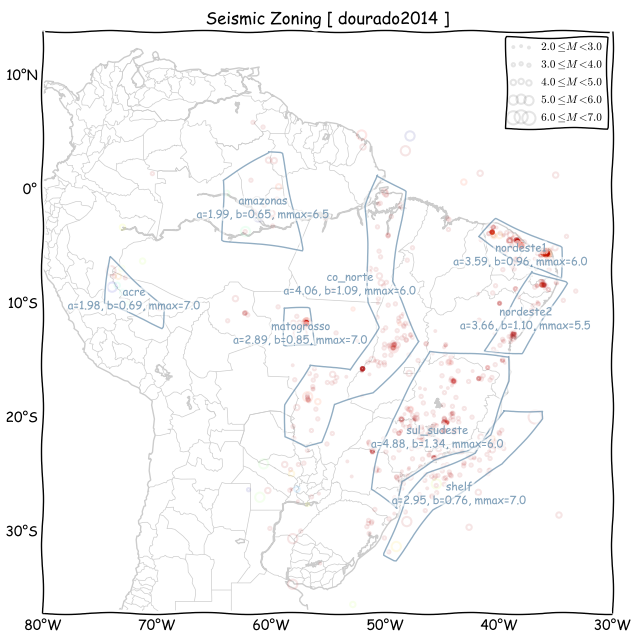
\includegraphics[width=.80\textwidth]{a_dourado} 
  \caption{Zoneamento sísmico e caracterização das zonas sísmicas por \citep{dourado_2014}.
  Os valores para a magnitude mínima foram de 3.0}
  \label{fig:a_dourado} 
\end{figure}

As zonas sísmicas foram apresentadas em detalhe de sismicidade e geologia no capítulo \ref{cap:regiao_de_estudo}.

O cálculo feito por Dourado com o programa Crisis \citep{crisis_2007} gerou os resultados da figura \ref{fig:pga_dourado}
para o mapa de ameaça sísmica (PGA, poe 10\% em 50 anos). Os valores originais \emp{Gal} $[cm/s^2]$ foram convertidos
para unidades de \emph{g} $[m/s^2]$.

\begin{figure}[H]
  \centering
  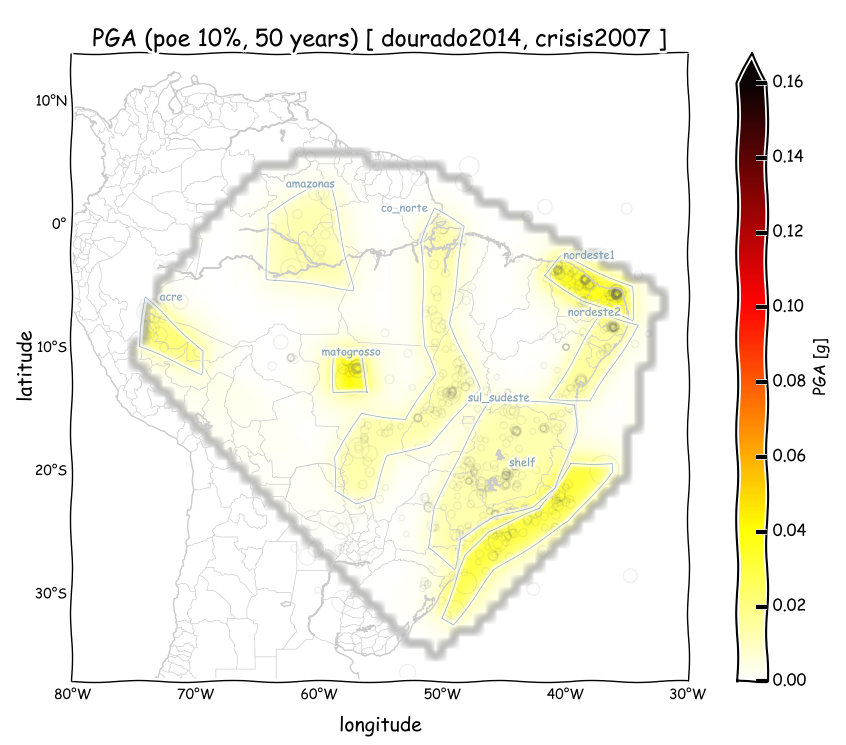
\includegraphics[width=.80\textwidth]{pga_dourado_crisis} 
  \caption{Resultado de \citet{dourado_2014} para o Brasil: PGA (10\%/50anos) em unidades de $g$ calculadas com o programa
  Crisis-2007}
  \label{fig:pga_dourado} 
\end{figure}

As mesmas fontes sísmicas e suas respectivas características foram utilizadas para o cálculo no
Openquake e os resultados estão apresentados na figura \ref{fig:pga_dourado_oq}.

\begin{figure}[H]
  \centering
  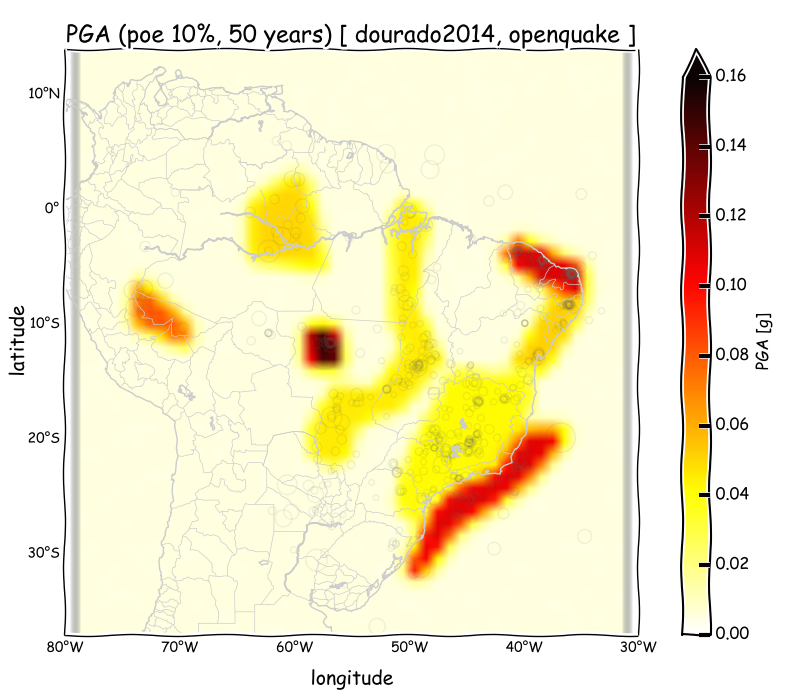
\includegraphics[width=.80\textwidth]{pga_dourado_oq} 
  \caption{Mapa de ameaça sísmica, PGA(poe 0.1, 50y)[Dourado, 20014] OpenQuake-Engine }
  \label{fig:pga_dourado_oq} 
\end{figure}

Os resultados preservam as feições mas apresentam quantidade significativamente diferentes.


%% ------------------------------------------------------------------------- %%
\section{Suavização da Sismicidade}
\index{suavização da sismicidade}
\label{sec:suavizacao_resultados}

Os métodos avaliados resultaram nos mapas de \emph{valor-a} e de ameaça sísmica
que serão apresentados nessa seção.

%% ------------------------------------------------------------------------- %%
\subsection{Frankel, 1995}
\index{Frankel,1995!resultados}
\label{sec:frankel_resultados}

Como resultado do processamento apresentado na seção \ref{sec:proc_frankel},
com distância de correlação de 150km e utilizando-se do catálogo BSB,
a taxa de sismicidade suavizada gerada pelo modelo pode ser vista na figura \ref{fig:a_fran_br}.
\begin{figure}[H]
  \centering
  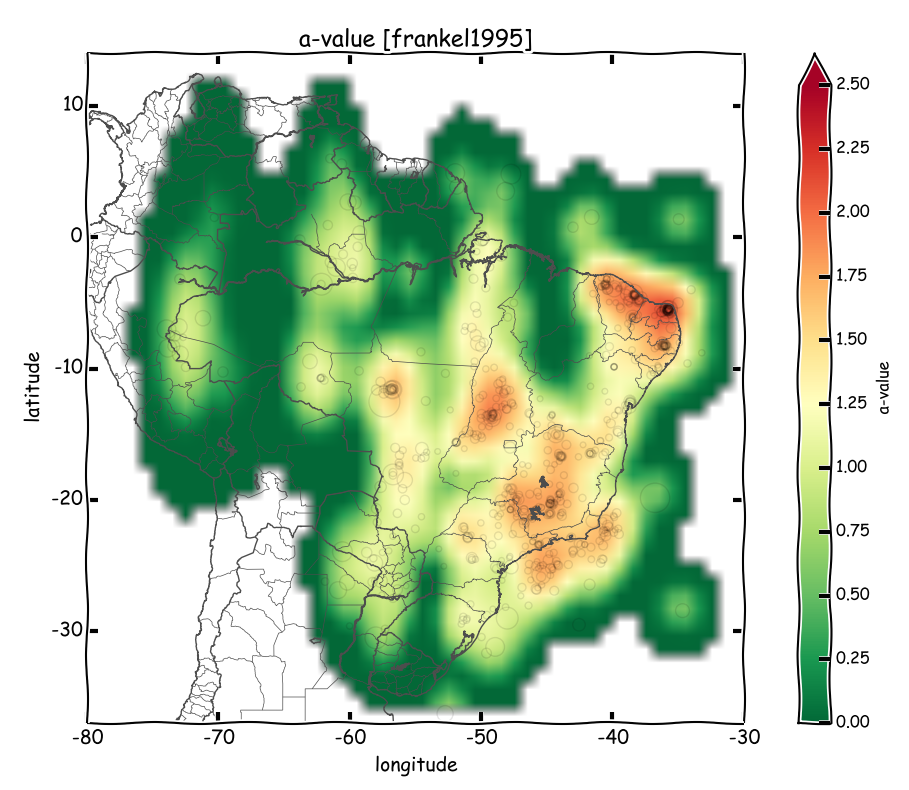
\includegraphics[width=.80\textwidth]{a_frankel_br} 
  \caption{Mapa do valor-a, usando o catálogo \gls{bsb2013} calculado pelo método de Frankel, 1995 }
  \label{fig:a_fran_br} 
\end{figure}

Apenas para comparação, o mesmo método foi empregado com o catálogo \gls{iscgem}, como pode ser visto na figura 
\ref{fig:a_fran_sa}.

\begin{figure}[H]
  \centering
  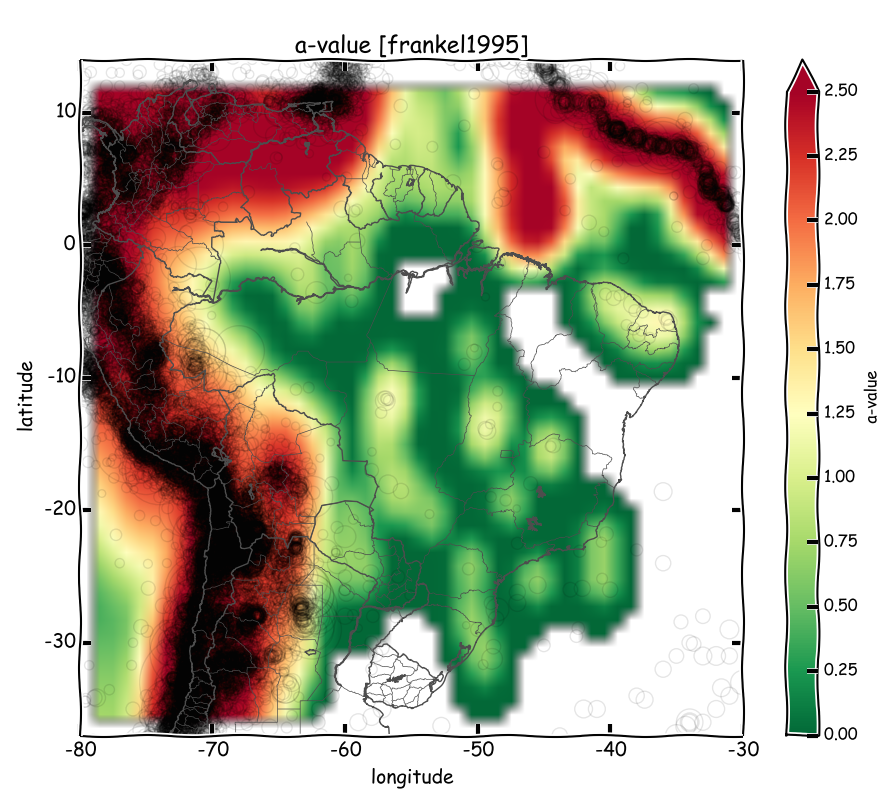
\includegraphics[width=.80\textwidth]{a_frankel_sa} 
  \caption{Mapa do valor-a, catálogo \gls{iscgem} [Frankel, 1995] }
  \label{fig:a_fran_sa} 
\end{figure}

Nos dois casos é possível perceber a compatibilidade entre os resultados na maior parte do Brasil, mas com
diferenças significativas na região do Acre, Rondônia e na porção norte na Dorsal Atlântica. 
Note que pela limitação da escala, os valores em vermelho são quaisquer valores acima de 2.5

Os valores da ameaça calculados conforme a seção \ref{sec:hazard} estão na figura \ref{fig:pga_fran}.

\begin{figure}[H]
  \centering
  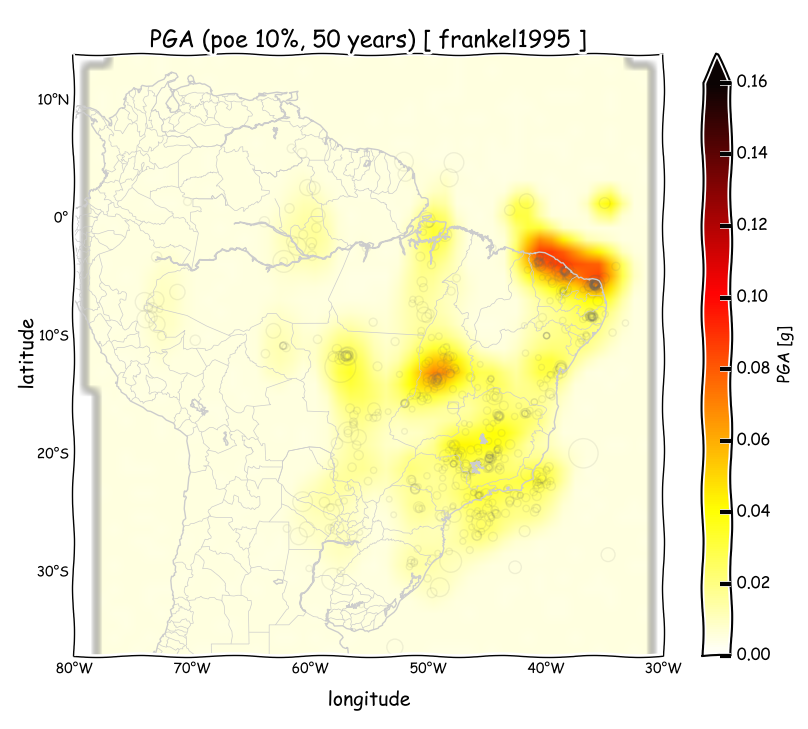
\includegraphics[width=.80\textwidth]{pga_frankel} 
  \caption{Mapa de ameaça sísmica, PGA (poe 10\%, 50y) [Frankel, 1995] }
  \label{fig:pga_fran} 
\end{figure}

Como técnica de suavização, é importante notar os principais altos de ameaça no nordeste e no centro do país.
A ameaça é recuperada razoávelmente na plataforma continental.

%% ------------------------------------------------------------------------- %%
\subsection{Woo, 1996}
\index{Woo, 1996!resultados}
\label{sec:woo_resultados}

O ajuste dos parâmetros da função de largura de banda resultou em $h(m)=1.39e^{1.18\,m}$.

Aplicando-se o método de Woo ao catálogo brasileiro desagrupado, a taxa de sismicidade suavizada 
pode ser avaliada pela figura \ref{fig:a_woo}.

\begin{figure}[H]
  \centering
  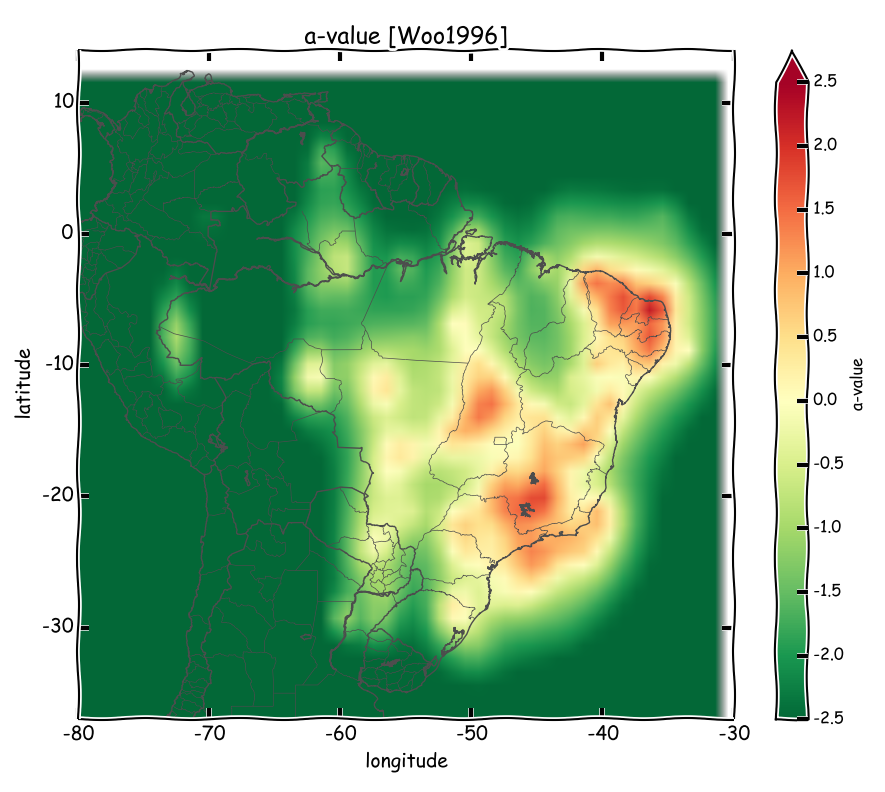
\includegraphics[width=.80\textwidth]{a_woo} 
  \caption{Mapa do valor-a, usando o catálogo \gls{bsb2013} calculado pelo método de Woo, 1996 }
  \label{fig:a_woo} 
\end{figure}

A sismicidade de regiões como o nordeste, Goiás/Tocantins, sudeste e plataforma continental 
foram bem recuperadas, enquanto partes da região norte e centro-oeste não tiveram tanto destaque. 

O cálculo da ameaça (figura \ref{fig:pga_woo_inc}) foi feito com o resultado direto do método, utilizando
diretamente uma \gls{mfd} discreta.
\begin{figure}[H]
  \centering
  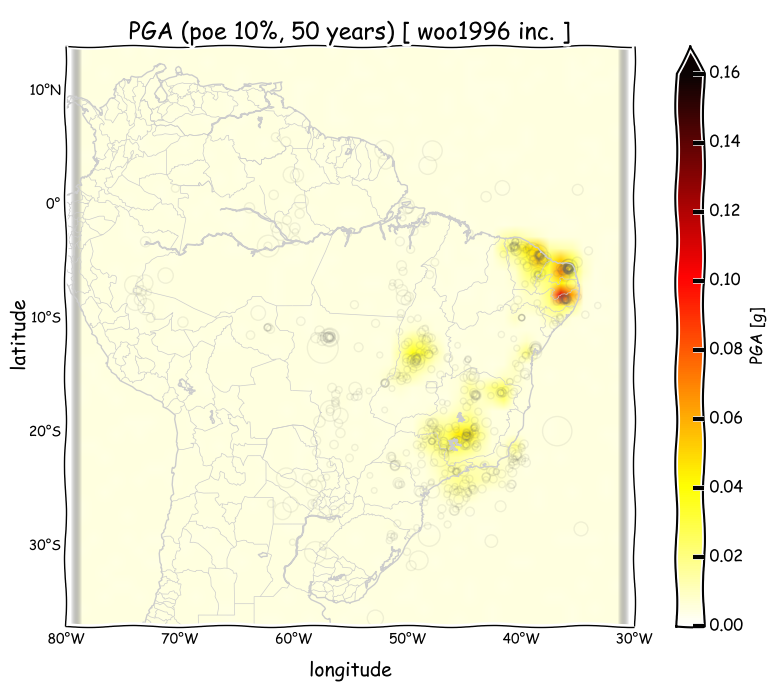
\includegraphics[width=.80\textwidth]{pga_woo_inc} 
  \caption{Mapa de ameaça sísmica, PGA (poe 10\%, 50y) 
  		   calculado com o Openquake a partir das fontes sísmicas
  		   determinas pelo método de Woo, 1996, usando uma \gls{mfd}
  		   discreta e incremental.
  }
  \label{fig:pga_woo_inc} 
\end{figure}

Coerentemente com a taxa de sismicidade modelada, as regiões norte, oeste e sul do país quase não figuraram 
enquanto parte do sudeste, plataforma, Goiás e nordeste foram destacadas. Merece ser notado o maior valor de ameaça
localizado em Pernambuco, dentre as três principais regiões mais ameaçadas do nordeste.

Para quantificar as diferenças nos cálculos de ameaça em decorrência da \gls{mfd} utilizada, em seguida é apresentado o
mapa de ameaça (figura \ref{fig:pga_woo_cum}) calculado a partir das taxas geradas pelo modelo, mas utilizando-se do
acumulado nos valores de magnitude acima do mínimo do catálogo e aplicando a transformação de Gutemberg-Richter 
para obter o \emph{valor-a}.
\begin{figure}[H]
	\centering
	\begin{subfigure}[t]{0.47\textwidth}
		\centering
		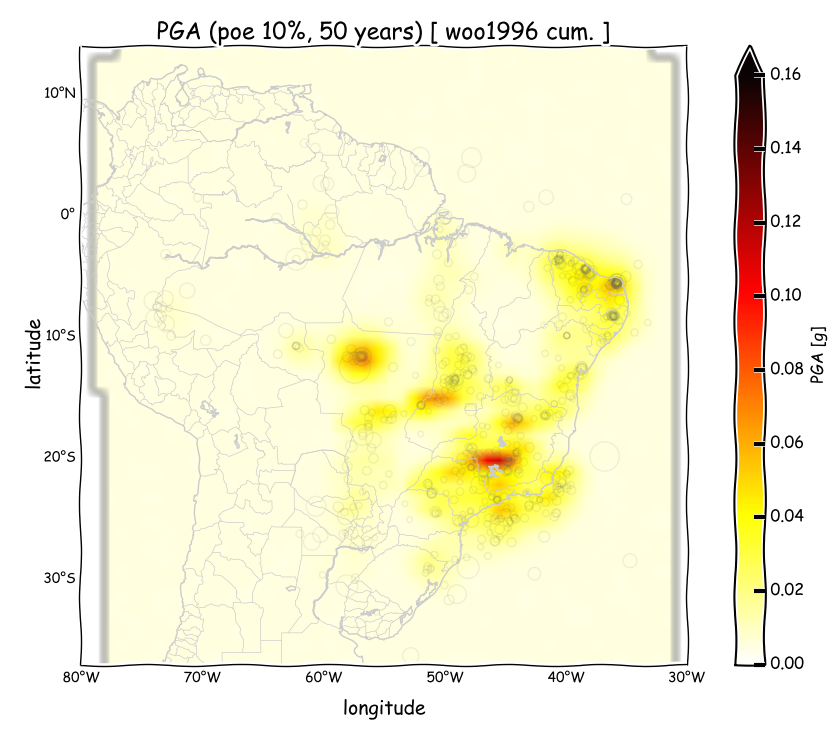
\includegraphics[width=1.0\textwidth]{pga_woo_cum} 
		\subcaption{Mapa de ameaça sísmica, PGA (poe 10\%, 50y), 
  		   calculado com o Openquake a partir das fontes sísmicas
  		   determinas pelo método de Woo, 1996, usando uma \gls{mfd}
  		   truncada usando o valor-a como o calor cumulativo
  		   contado a partir da \gls{sym:Mmin}.
		}
		\label{fig:pga_woo_cum} 
	\end{subfigure}
	\quad
	\begin{subfigure}[t]{0.47\textwidth}
		\centering
		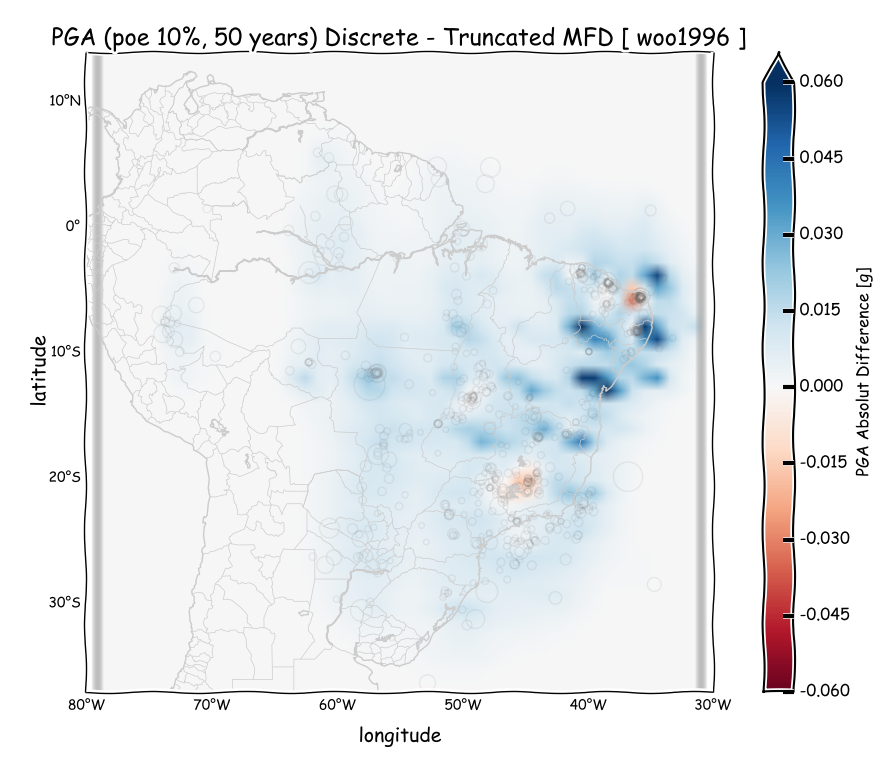
\includegraphics[width=1.0\textwidth]{pga_woo_dif} 
		\subcaption{Mapa diferencial de ameaça, PGA (poe 10\%, 50y), 
		   entre os modelos usando \gls{mfd} truncada e \gls{mfd}
		   discreta. Diferença entre os mapas das figuras 
		   \ref{fig:pga_woo_inc} e \ref{fig:pga_woo_cum}.
		   }
		\label{fig:pga_woo_dif} 
	\end{subfigure}
	\caption{Variação do resultado da ameaça em função do uso de diferentes 
			\glspl{mfd} no OpenQuake}
	\label{fig:pga_woo} 
\end{figure}

A figura \ref{fig:pga_woo_dif} quantifica a diferença nos valores de ameaça obtitos quando 
utilizadas as diferentes distribuições de frequência e magnitude. Nota-se que enquanto
o modelo com \gls{mfd} incremental destaca principalmente o nordeste, o modelo utilizando o \emph{valor-a}
cumulativo e uma \gls{mfd} truncada, destacou principalmente as ameaças no centro-oeste e sudeste.


%% ------------------------------------------------------------------------- %%
\subsection{Helmstetter, 2012}
\index{Helmstetter, 2012!resultados}
\label{sec:helmstetter_resultados}

A otimização dos parâmetros do modelo de Helmstetter conforme descrito na seção \ref{sec:proc_helmstetter}
resultou, com ganho\footnote{equação \eqref{eq:gain}} $G = 2.43$, nos valores apresentados na tabela
\ref{tab:hemlstetter}.

\begin{table}[H]
	\centering
	\begin{tabular}{c|c}
		Parâmetro & Valor \\ \hline
		$R_{min}$ & $0.1\times10^{-13}$ \\
		$a_{cnn}$ & 325 \\
		$k_{cnn}$ & 1 \\
	\end{tabular}
	\caption{Parâmetros otimizados para o modelo de Helmstetter a partir do catálogo \gls{bsb2013}}
	\label{tab:hemlstetter}
\end{table}

Usando os parâmetros otimizados, os valores calculados para a taxa de sismicidade
de longo-prazo pelo método proposto por Helmstetter pode ser visto na figura \ref{fig:helm_r}.

\begin{figure}[H]
  \centering
  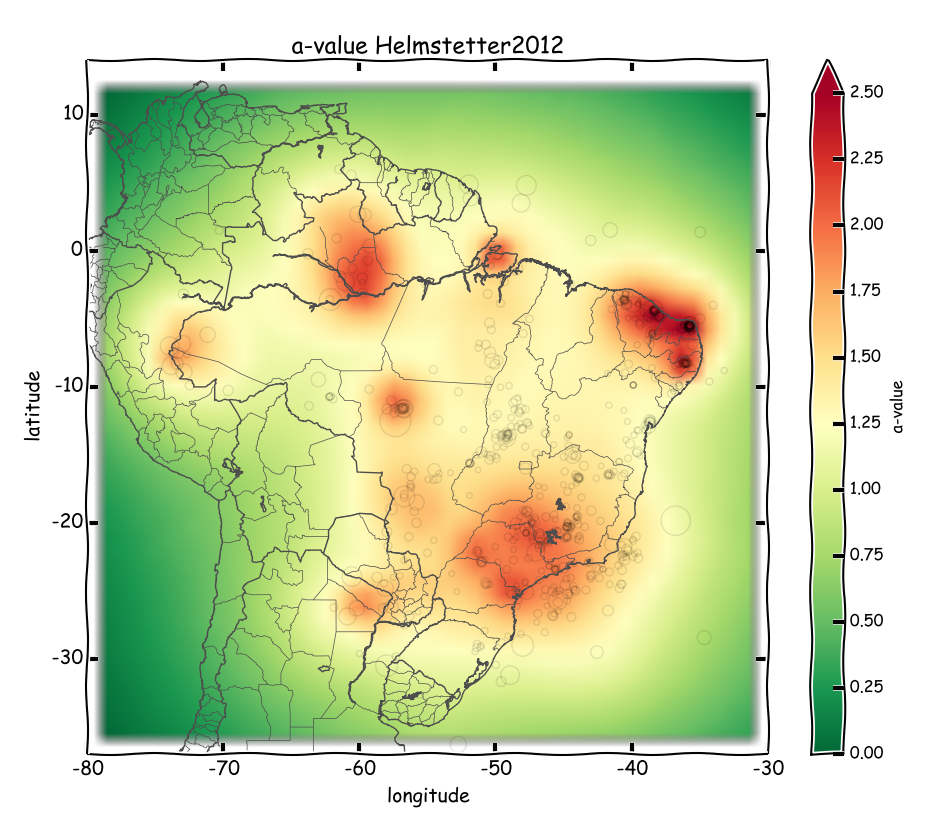
\includegraphics[width=.80\textwidth]{a_helmstetter} 
  \caption{Mapa do valor-a, usando o catálogo \gls{bsb2013} calculado pelo método de Helmstetter, 2012 }
  \label{fig:helm_r} 
\end{figure}

Observa-se que a sismicidade de regiões como amazônia, Mato-Grosso e Pará foram destacadas,
enquanto no sudeste houve maior diluição. A sismicidade do nordeste aparece evidente, principalmente
nas regiões do Ceará, Rio Grande do Norte e Pernambuco.

Na figura~\ref{fig:helm_h} estão os valores calculados para o mapa de ameaça 
com as taxas de sismicidade suavizadas pelo método.

\begin{figure}[H]
  \centering
  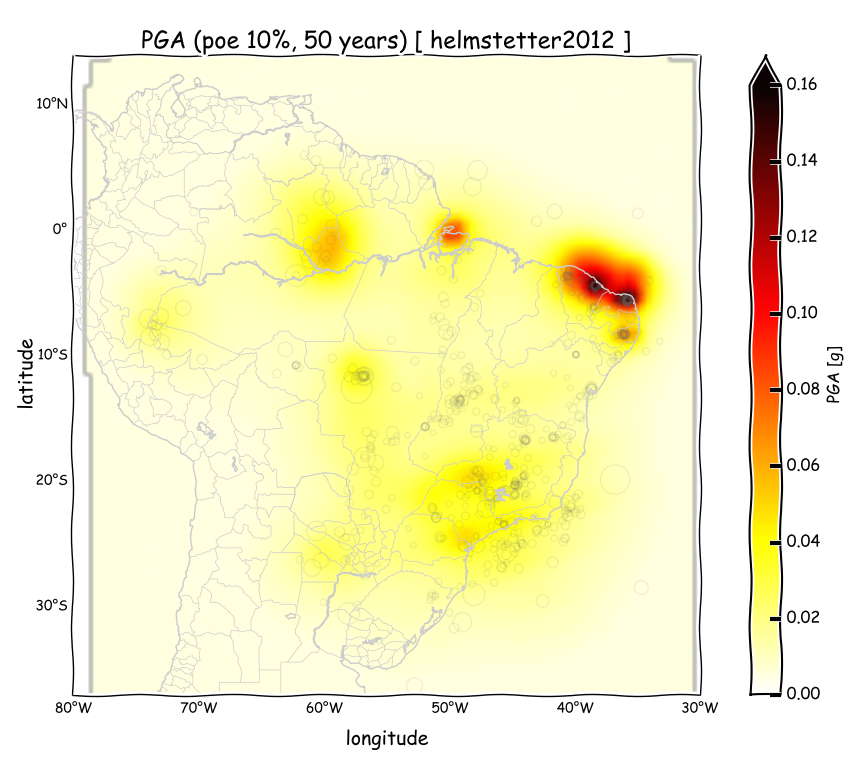
\includegraphics[width=.80\textwidth]{pga_helmstetter} 
  \caption{Mapa de ameaça sísmica, PGA (poe 10\%, 50y), 
  		   calculado com o OpenQuake a partir das fontes sísmicas
  		   determinas pelo método de Helmstetter,2012 }
  \label{fig:helm_h} 
\end{figure}

Nota-se que ao passo em que houve um grande realçe da ameaça em algumas regiões como amazônia e Pará (próximo a Belém),
em regiões como a faixa sísmica no norte de Goiás e Tocantins não apresentaram o mesmo contraste.


